Value Iteration is a algorithm used to compute an optimal policy in a \textbf{Markov Decision Process (MDP)}. It iteratively updates state values to approximate the optimal value function, which determines how good it is to be in a particular state. \vspace{10pt}

\noindent The algorithm is based on the \textbf{Bellman Optimality Equation}, which defines the relationship between the value of a state and the expected rewards of possible future states. The update rule is defined as:

\begin{equation}
    V(s) \leftarrow \max_{a} \sum_{s'} P(s'|s, a) \left[ R(s, a, s') + \gamma V(s') \right]
    \label{eq:bellman}
\end{equation}

where:
\begin{itemize}
    \item $V(s)$ represents the value of state $s$.
    \item $P(s'|s, a)$ is the transition probability of reaching state $s'$ from $s$ by taking action $a$.
    \item $R(s, a, s')$ is the immediate reward received when transitioning from $s$ to $s'$ via action $a$.
    \item $\gamma \in [0,1]$ is the discount factor, which determines how much future rewards influence current decisions.
\end{itemize}

\noindent \textbf{Value Iteration Algorithm:} The process begins with arbitrary initial values for $V(s)$. In each iteration, the values are updated using Equation~\eqref{eq:bellman} until they converge within a predefined threshold $\epsilon$. This ensures that the values stabilize close to the optimal value function. Once convergence is achieved, the optimal policy $\pi^*(s)$ can be derived by selecting the action that maximizes the expected utility:

\begin{equation}
    \pi^*(s) = \arg\max_{a} \sum_{s'} P(s'|s, a) \left[ R(s, a, s') + \gamma V(s') \right]
\end{equation}

\noindent The pseudocode for the Value Iteration algorithm is provided below.

\begin{algorithm}
\caption{Value Iteration}
\label{alg:value_iteration}
\begin{algorithmic}[1]
    \Function{VALUE-ITERATION}{$mdp, \epsilon$}
        \State \textbf{inputs:} $mdp$, an MDP with states $S$, actions $A(s)$, transition model $P(s'|s, a)$,
        \State \hspace{1.6cm} rewards $R(s)$, discount $\gamma$
        \State \hspace{1.6cm} $\epsilon$, the maximum error allowed in the utility of any state
        \State \textbf{local variables:} $U, U'$, vectors of utilities for states in $S$, initially zero
        \State \hspace{1.6cm} $\delta$, the maximum change in the utility of any state in an iteration
        \Statex
        \Repeat
            \State $U \gets U'$
            \State $\delta \gets 0$
            \For{each state $s \in S$}
                \State $U'[s] \gets R(s) + \gamma \max_{a \in A(s)} \sum_{s'} P(s'|s, a) U[s']$
                \If{$|U'[s] - U[s]| > \delta$}
                    \State $\delta \gets |U'[s] - U[s]|$
                \EndIf
            \EndFor
        \Until{$\delta < \epsilon(1 - \gamma)/\gamma$}
        \State \Return $U$
    \EndFunction
\end{algorithmic}
\end{algorithm}

\subsection{Description of Implemented Solution}
This section details the implementation of the Value Iteration algorithm. The Python implementation follows the pseudocode in Algorithm~\ref{alg:value_iteration}. Since the problem does not define terminal states and the agent’s state sequence is infinite, we estimate the upper bound of a tile’s utility using the geometric series:

\begin{equation}
    \text{Max Utility} \approx S_{\infty} = \frac{1}{1 - 0.99} = 100
\end{equation}

\noindent Experimental results later confirm that the computed values are consistent with this estimate. Additionally, due to the absence of a fixed trajectory, the optimal policy remains independent of the agent’s starting position. \vspace{10pt}

\noindent The Value Iteration algorithm implemented in Figure ~\ref{alg:value_iteration} follows a \textbf{synchronous approach} where 2 copies of the value map as seen in line 122. \vspace{10pt}

\noindent Each state is updated with the \textbf{Bellman Equation} as seen in lines 128 to 134. \texttt{actionl} is a list of actions and \texttt{probs} is a list of the respective action's probabilities. \vspace{10pt}

\noindent We subsequently use the actions to obtain the next state $S_{t+1}$ and reward $r$ via the \texttt{step} method, and update the values of each state with the \textbf{Bellman Equation}. \vspace{10pt}

\noindent Next, in lines 136 - 141, the max value over all actions is saved as the value of the current state, while the action that produced the max value is saved as the policy. \vspace{10pt}

\noindent In line 145, we track and store the historical state values for plotting and analysis. \vspace{10pt}

\noindent The iteration then continues until the max difference across all states between the old and the new best values is $\Delta \leq \Theta$ where $\theta$ is a small user-specified positive value, indicating that the algorithm is approaching convergence. In our implementation, we use a value of $\theta = 0.001$ resulting in 688 iterations needed to reach convergence. 

\begin{figure}[H]
    \centering
    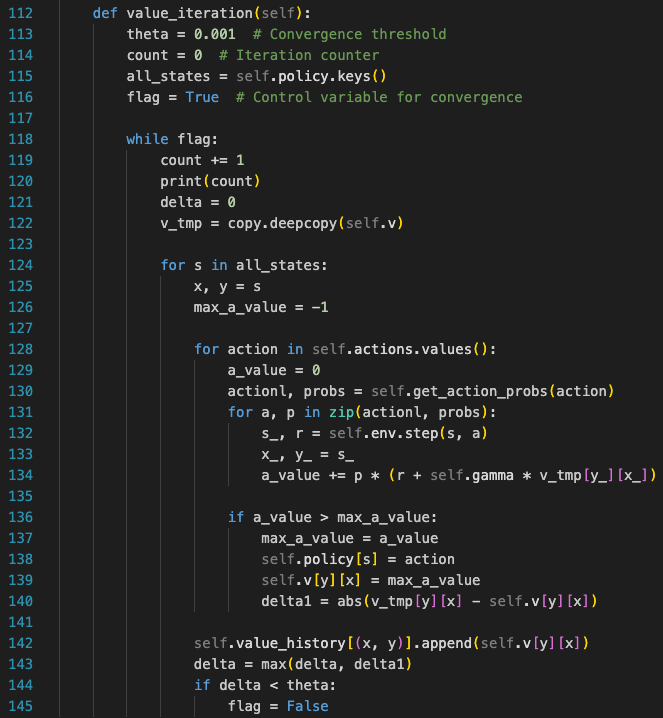
\includegraphics[width=0.8\textwidth]{images/vi_impl.png}
    \caption{Value Iteration Implementation}
\end{figure}

\subsection{Plot of Optimal Policy}
After executing the Value Iteration algorithm, the computed optimal policy is displayed as console output, representing the direction of movement for each state:

\begin{figure}[H]
    \centering
    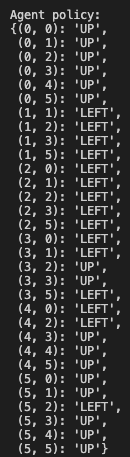
\includegraphics[width=0.2\textwidth]{images/vi_policy.png}
    \caption{Console Output of Value Iteration Policy}
\end{figure}

To enhance intepretability, we generate a plot of the optimal policy:

\begin{figure}[H]
    \centering
    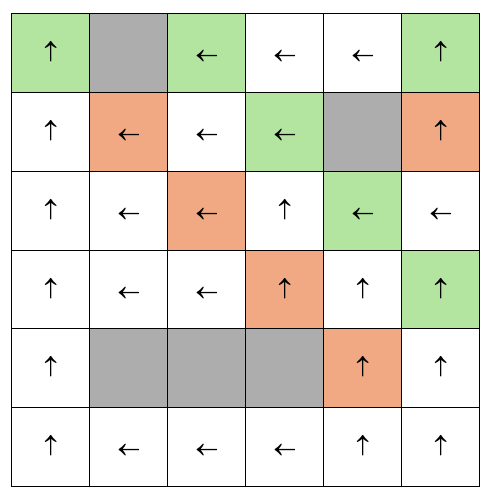
\includegraphics[width=0.6\textwidth]{images/vi_plot_policy.png}
    \caption{Plot of Optimal Policy}
    \label{fig:vi_plot_policy}
\end{figure}

\noindent Figure~\ref{fig:vi_plot_policy} provides a structured visualization of the agent's decision-making process. We observe that the agent predominantly moves \textbf{towards the top-left corner}.

\subsection{Utility of All States}
As shown in Figures ~\ref{fig:vi_console_utility} and ~\ref{fig:vi_plot_utility}, the computed utilities closely align with the estimated upper bound of approximately 100, confirming the accuracy of the Value Iteration algorithm in converging to the expected utility values.

\begin{figure}[H]
    \centering
    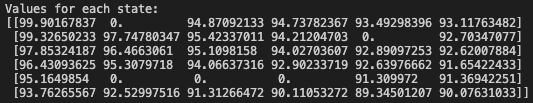
\includegraphics[width=0.8\textwidth]{images/vi_utility.png}
    \caption{Console Output of Value Iteration Utilities}
    \label{fig:vi_console_utility}
\end{figure}

\begin{figure}[H]
    \centering
    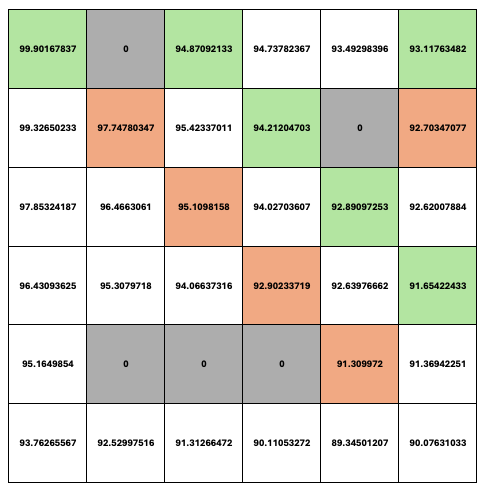
\includegraphics[width=1.0\textwidth]{images/vi_plot_utility.png}
    \caption{Plot of Utilities of All States}
    \label{fig:vi_plot_utility}
\end{figure}

\subsection{Plot of Utility Estimates as a Function of the Number of Iterations}
As previously mentioned, we set the convergence threshold $\theta$ to 0.001. Consequently, the Value Iteration algorithm required a total of 688 iterations to reach convergence. Figure ~\ref{fig:vi_plot_utility_est} illustrates the progression of utility estimates as a function of the number of iterations, highlighting the algorithm's stability and convergence behavior.

\begin{figure}[H]
    \centering
    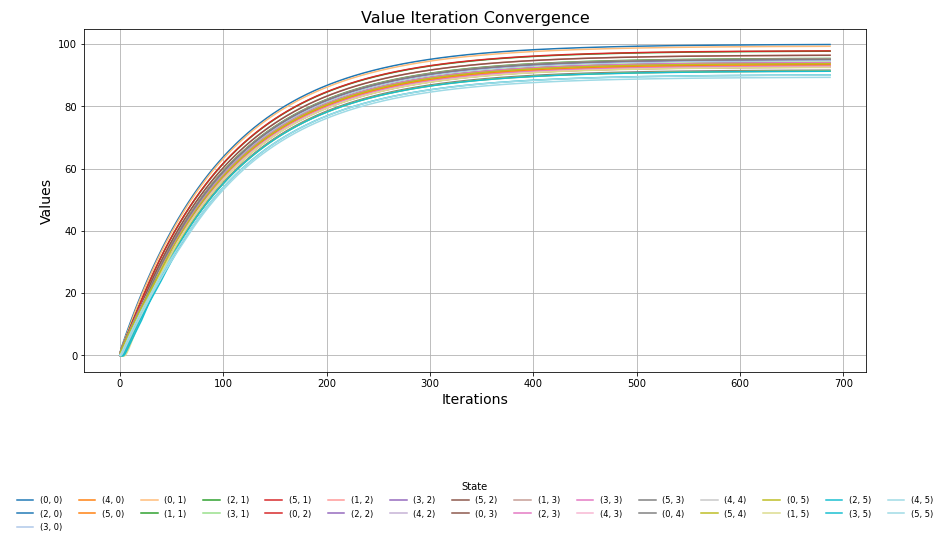
\includegraphics[width=1.0\textwidth]{images/vi_plot_utility_est.png}
    \caption{Plot of Utilities Estimates as a Function of the Number of Iterations}
    \label{fig:vi_plot_utility_est}
\end{figure}
